% Chapter 3 - Methodology
%	Research of Current Tools
%	Development
%		Prototyping elements
%	Testing
%	Further Development
%		Small optimisations
%		Discuss assumed future work
%- Guide (1250-2000 Words)

\chapter{Methodology}
\label{chap:chapter3}
This investigation was split into three sections, all of which are further split into subsections.
The three objectives that were in focus were: Research of current tools, Development, and a Final Analysis.

\section{Research of String Searching Algorithms}
A great deal of time was spent in researching String searching algorithms that would be fit for this purpose.
Existing tools favour the use of the \acf{BM} algorithm.

\subsubsection*{\acl{BM}}
\acf{BM} makes use of two rule sets in order search through a string while skipping areas sections that the algorithm deem non applicable.
As these rules can perform jumps without needing to know the contents of the text they are often implemented to be pre-processed.
When the algorithm encounters a character outwith the pattern it can jump via one of the two rules:
\begin{itemize}
    \item Bad Character: Upon mismatch the BM will skip alignments until either; a mismatch becomes a match or the pattern moves past the mismatched character.
\begin{figure}[!ht]
    \centering
    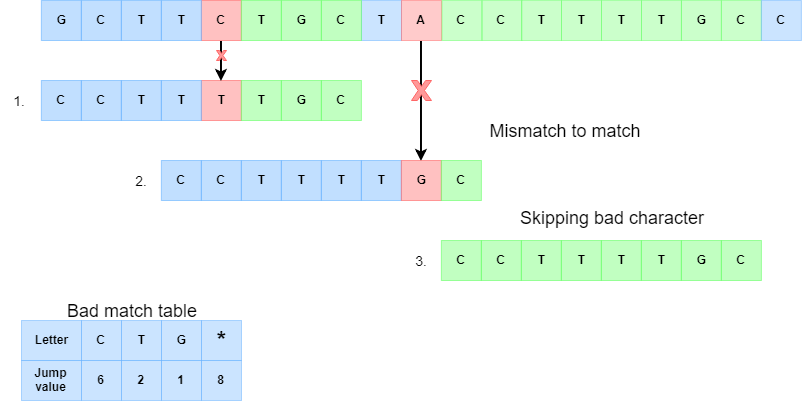
\includegraphics[width=\linewidth]{Images/BMBadMatch.png}
    \caption{Visualisation of the \acl{BM} bad match rule}
    \label{fig:BM_BadMatch}
\end{figure}
\newpage    
    \item Good Suffix: In searching the string when only a partial match is reached a search is then performed within the pattern to see if any sub-string of this partial match can exist in the pattern. 
\begin{figure}[!ht]
    \centering
    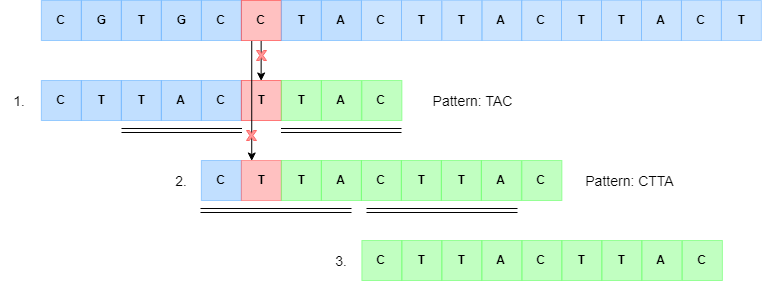
\includegraphics[width=\linewidth]{Images/BMGoodSuffix.png}
    \caption{Visualisation of the \acl{BM} good suffix rule}
    \label{fig:BM_GoodSuffix}
\end{figure}
\end{itemize}

When searching for a string \ac{BM}, typically, starts the patterns length into the string and reads patterns from their last character as they are discovered; right to left.
This can also be an issue as some of the patterns that are being searched for end with the default hex character on a empty disk {\textbackslash}x00.

As these jump tables are generated by \ac{BM} for each pattern, multiple searches through the string are required to find every pattern.
It would also be considered inefficient to implement BM into a functional algorithm for use on a GPGPU device for architectural difference to CPU that will be later explained. Due to GPGPU assets' much higher core count -- compared to CPU -- and independent memory a different approach to string searching is required to operate at a higher efficiency.

\subsubsection*{\acl{AC}}
The \acf{AC} method of string searching makes use of a pattern trees (tries) to navigate its search of many strings.
Using the state machine design from Knuth-Morris-Pratt, with said pattern tree, multiple strings can be searched for simultaneously.
This method results in almost no reduction in efficiency when attempting to search for multiple patterns.
\ac{AC} is also able to double back on itself within the tree where a pattern ceases but the potential of a different pattern exists; this functions similar to the good suffix rule previously discussed but would be better explained as a pointer to a different section of the search.
A visualisation of the jump table as explained can be seen in Figure \ref{fig:AC_diagram} will hopefully supplement the explanation.
\newpage
\begin{figure}[!ht]
    \centering
    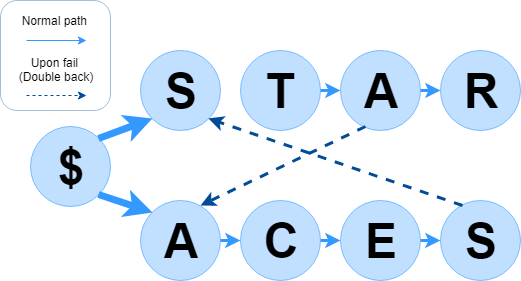
\includegraphics[width=240pt]{Images/AC_Visualisation.png}
    \caption{Visualisation of the \acl{AC}}
    \label{fig:AC_diagram}
\end{figure}
\subsubsection*{\acl{PFAC}}
\label{sec:PFAC}
\acf{PFAC} is the reduced version of \ac{AC}.
By removing the “Double Back” Failure states as seen in Figure \ref{fig:AC_diagram}, execution of the algorithm will simply cease in the event of a non-pattern.
This makes the algorithm more applicable for GPGPU architecture, where the intent would be to run the algorithm on many cores simultaneously and each thread of execution should remain as simple as possible.

\section{Research of current tools}
Before tests into the benefits provided by GPGPU methods can be developed, existing tools must be researched and a baseline must be established.
Unlike the methods in the paper ``Performance analysis of file carving tools’’ (Laurenson, 2013), the metrics being gathered for this will entirely be based on timings and data throughput.

Research for this investigation was focused into file carving tools that currently exist in open source; as these tools clearly showed how they operated.
Comparison between these tools allowed for great insight into favourable design practices, along with an understanding as to how the entire process of file carving is currently performed.
Analysis of these tools helped with identification into a platform to expand upon; although this decision concluded to not expand an existing platform but instead develop a new one for the purposes of testing.

From this and the literature that was reviewed, sufficient knowledge to develop this project was gained in the subject areas of; file carving, string searching, hardware and software design practices.
Multiple means of development were considered and one particularly difficult design choice was made during this stage between GPGPU \ac{API}s.

\subsubsection*{GPGPU Programming Libraries}
Before development could begin the choice of which \ac{GPGPU} \acf{API} should be used was considered.
This was between the options: CUDA or OpenCL.
This choice between the \acp{API} was made to ensure the right balance is being met between; ease of product development, delivery to multiple platforms, and \ac{API} performance.

The CUDA platform has the benefit of being simpler, thus easing product development, and having many optimisations as it is built for a specific subset of hardware.
The latter point comes with its disadvantages as CUDA is limited to Hardware distributed by NVidia.

The OpenCL platform is Open Source and developed for many hardware types which makes the final product more accessible, thus available to more systems.
Performance, although less efficient, can be made up from CUDA by making use of the \acf{IGP}.
The disadvantage here is in the time it will take to develop for this platform due to its complexity.

As such, it was decided that between these two platforms CUDA should be used and development of the final product was executed using this \ac{API}.

\section{Development}
Once the main body of research was complete and the foundation was decided upon, development could begin using C++ with the CUDA \ac{API}.
This language has its benefits in the researchers perspective due to previous knowledge of not only the syntax but of the and high efficiency the code can compile to meet.
As the existing tools, Scalpel and Foremost, make use of C and C++ they were used as a reference as to how to perform certain actions.
Furthermore, where these examples lacked, both C++ and the CUDA \ac{API} have readily available and verbose documentation -- not to mention large presences on Stack Overflow -- that could assist in the implementation process.

\subsubsection*{\acl{RAD}}
As it was expected that a great deal of time would be spent in the tool testing and development, this appeals to a methodology that makes use of proto\-typing.
As such the \acf{RAD} model was chosen. The \ac{RAD} methodology can be seen in Figure \ref{fig:RAD}.

\begin{figure}[!ht]
    \centering
    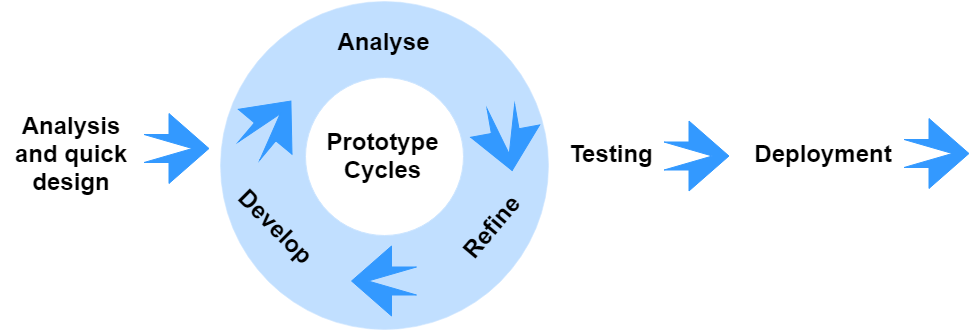
\includegraphics[width=230pt]{Images/RAD.png}
    \caption{\acl{RAD} Model}
    \label{fig:RAD}
\end{figure} 

By allowing testing to be performed during development, comparisons between all of the branches/prototypes test metrics would reveal where the development should continue.
This also subsequently helped to reveal many avenues of Future work.

\subsubsection*{Development environment setup} % These were used for the testing
In order to begin programming after decisions were made as to how to proceed, an environment was required that allowed for the compilation and execution of CUDA code.
CUDA makes use of it's own compiler, the NVidia C Compiler (NVCC), and although this can be installed without CUDA assets installed it is not typically recommended.
Two methods were employed to assist in the compilation and execution of CUDA code: NSight for Visual Studio (Windows) and the NVidia CUDA Toolkit (for Ubuntu).
Both of these had their merits as they each Operating system had tools that would be compared against that were native to them.

Each environments hardware specifications were taken to provide more insight and clarification as to the results of each test.
Tests that were made on one environment should not be compared to those from another due to the major differences that exist between them.
\acf{AWS} was used for testing to allow for the recreation of results.
By using this hardware/instance template any user should be able to access the same environment during their own testing.

{\centering
\begin{tabular}{c | c | c}
& Environment A & Environment B \\
& Personal Desktop & AWS g3s.xlarge \\
\hline
CPU & 4 Core, i5 3570k & 4 vCore's, Xeon E5-2686 v4 \\
\hline
GPU & GTX 980 Ti & TESLA M60 \\
\hline
Memory & 16\ac{GB}, 1333MHz & 30.5\ac{GB} \\
\hline
Backing Storage & \ac{SSD}, ?\ac{MB}/s & \ac{SSD}, 107\ac{MB}/s \\
\hline
\ac{OS} & Windows & Ubuntu Server 18.04 \\
\end{tabular}
\captionof{table}{Testing Environment Specifications}
\label{tab:TestingEnv}
\par}

Environment A's Backing storage speed is undetermined as the tool that was used to measure it returned improbable results for read speeds.
The given result suggested that reads could take place at 2483.00 MiB/s (2603.614 \ac{MB}/s) where the maximum theoretical bandwidth possible for a SATA III device is 600\ac{MB}/s.
These results were taken via the tool \href{https://github.com/Microsoft/diskspd}{diskspd.exe} and it is assumed that the developers really meant Megabits (Mb) which would result in 310.4MB/s.
This issue was clearly brought about by the inconsistent standard for what MiB stands for so the true limit of the disk was unestablished but the highest recorded speed was 390.27MB/s.

Now with access to the CUDA Compiler now established on two machines and their specifications known, implementation could proceed.

\subsubsection*{Implementation}
The development of the program was split into sections that could operate autonomously, thanks to the use of object oriented programming.
These compartmentalised sections were the file chunking method and the string searching method.
Both of these were designed independently due to the benefits that are provided when testing the code for both syntax and logical errors.
When searching for errors in the file chunking method this technique especially proved its worth but this will later be discussed.

The \ac{PFAC} string search was another key part of this implementation.
This search was designed through multiple iterations from single-threaded \ac{CPU} right up to multi-threaded \ac{GPU}.
The complete search could be identified as two different sections, the \ac{PFAC} search tree and the \ac{PFAC} search.
Referencing the OpenForensics code, written in C\#, this algorithm was implemented.

\section{Final Analysis}
Although analysis was performed throughout the development cycle the gained results were not not directly compared with other file carvers in a quantitative manner.
As such, the final analysis included direct comparisons between the final prototype and these existing file carvers while they are set to audit for files but not carve them.
This process took extra steps to accommodate the differences present between each tool analysis.

Test images were generated for this containing files known to the researcher.
As such the researcher was able to accurately test these tools for false positives and negatives as they knew exactly what results are to be expected with headers and footers.

After testing against other tools the processing rates of each chunk once it has been provided to the \ac{GPU} was subject to comparison followed by the data throughput.
Data Throughput of the program will be compared to the `theoretical maximum' (Bayne, 2017); the theoretical maximum in this context is in reference to the backing storage's ability to provide the data -- Disk Image Chunks –- to search.
This testing was performed multiple times to reduce the chance of `jitter' (Bellekens et al., 2017) effecting the results integrity.

As not all tools were able to be ran on the same system -- mostly due to the \ac{OS} compatibility of each – test results were only compared to other results on the same system.
Development as a result kept focus on the likely use on multiple devices and did not focus development to one system configuration.

% \section{Further Optimisations}
% Even during the process of development it was clear that some sections should be removed from the realm of expectation and assigned as future work.
% Only through complete trust of the theoretical design of the final product was this easy to distinguish.
% This is why much of the time distributed in this investigation was to gaining an understanding of existing file carvers.
% Many of these aspects that were future work however were items that could in fact easily be implemented.
% It is because of this optimisations were not expected to make it into the final product were able to be made throughout the development.
% Sections that were initally considered as future work will be discussed as they are discussed.